% (c) Jakub Stejskal
% Master Thesis
% Performance Testing and Analysis of Qpid-Dispatch Router
% Chapter 6

\chapter{Experimental Evaluation}
\label{Experimental Evaluation}
This chapter summarizes collected results during the performance testing with Messaging Performance Tool. We decided to split the testing into two parts. The first part is basic measurement with version of Maestro 1.2.4. During this measurements we were finding higher possible throughput of singlepoint topology of Qpid-dispatch and multipoint topology with three nodes of Qpid-dispatch or with Broker in the middle. The topologies are depicted in the image \ref{fig:excel_throughput}. The second series of measurement was focused on behavior testing of the topologies. For this measurements, we used Maestro version 1.3.0 which includes Maestro Agent and AMQP Inspector.

Since the testing was done over multiple topology types, we used Topology Generator for quick automatic topology changes. All measurements was orchestrated by an automation server called Jenkins\footnote{Jenkins\,---\,\url{https://jenkins.io/}}.

\section{Basic Performance Measurements}
\label{Basic Performance Measurements}
Maestro works as the orchestration system, I needed proper infrastructure before I could run any test for our experimental evaluation. The architecture of Maestro, described in the Chapter \ref{Messaging Performance Tool}, specifies that in ideal scenario I need at least four machines for running a simple test: maestro broker, sender, receiver, and SUT. The amount of needed machines rises with more complex scenarios and larger network. Examples of generated topologies are depicted in the Figure \ref{fig:basic_topologies}. For both of these configurations I compared the throughput and latency of these combinations and discuss the results with supervisors and author of MPT. The results of this measurements was described and published in the paper for Excel@FIT\footnote{Excel@FIT\,---\,IT conference for students and theirs work \url{http://excel.fit.vutbr.cz/}} conference.

\begin{figure}[h]
	\centering
	\begin{minipage}{0.45\linewidth}
		\subfloat[Topology consists of routers.\label{fig:basic_topology_router}]{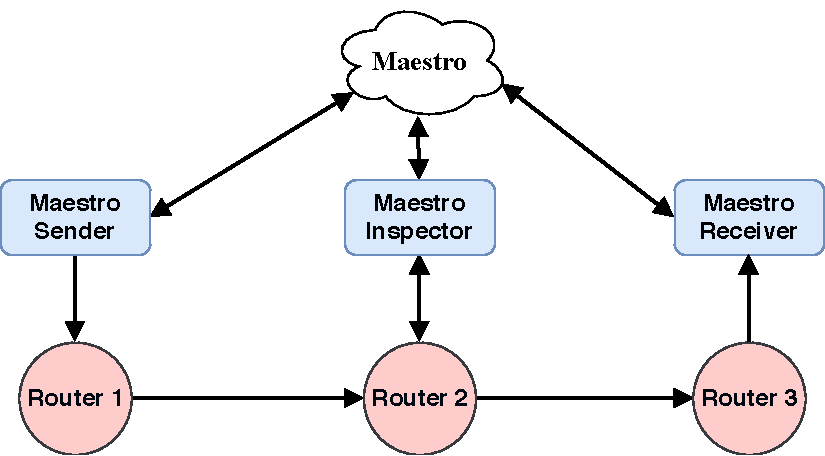
\includegraphics[width=\linewidth]{obrazky-figures/basic_topology_router.pdf}}
	\end{minipage}
	\begin{minipage}{0.45\linewidth}
		\subfloat[Topology with Broker in the middle.\label{fig:basic_topology_broker}]{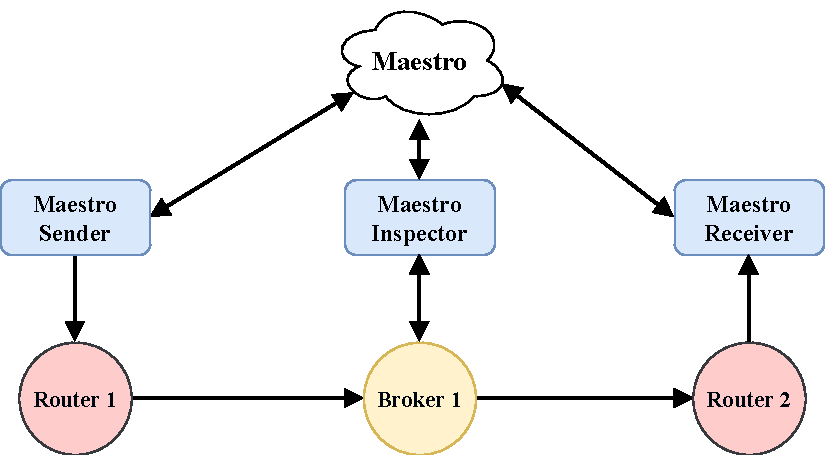
\includegraphics[width=\linewidth]{obrazky-figures/basic_topology_broker.pdf}}
	\end{minipage}
	\caption[A simple network with active router agent.]{Topologies created for basic performance testing.}\label{fig:basic_topologies}
\end{figure}

\subsection{Throughput}
\label{Throughput}

\begin{figure*}[h]
	\centering
	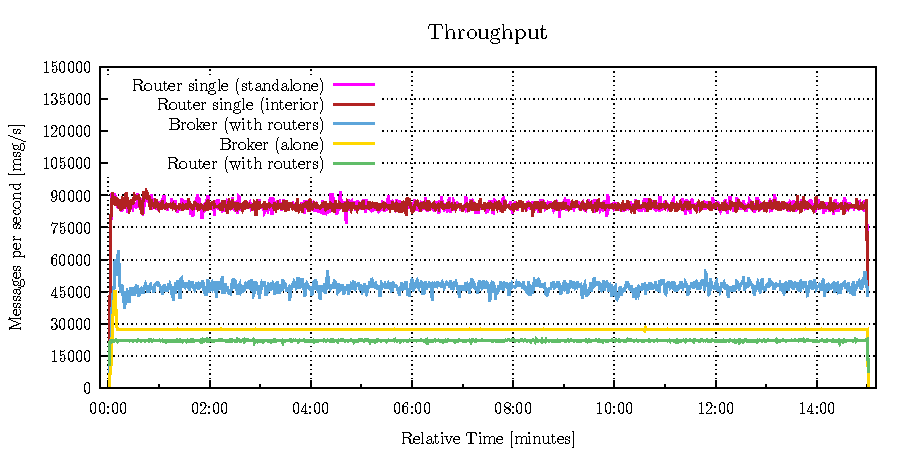
\includegraphics[width=1\linewidth]{obrazky-figures/charts-excel/throughput.pdf}
	\caption{Chart of maximum throughput of router and broker during specific test cases.}
	\label{fig:max_rate}
\end{figure*}

I measured throughput only by load generators\,---\,\emph{Maes\-tro Sender} and \emph{Maestro Receiver}. Load generation depends on the test properties. Maestro is able to create unbounded rate test, during which it generates as much load as it can. This type of test was used to reach maximum handled rate of Qpid-dispatch and its result is depicted in the Figure \ref{fig:max_rate}. However, the maximum rate was not achievable on all topology types. Qpid-dispatch offers two modes\,---\,\emph{standalone} and \emph{interior}, where standalone works as single router machine in the network, while interior type works with multiple routers. The current version of Qpid-dispatch has an ability to load balance when buffers are almost full. This ability offers faster message delivery in cost of a slower throughput. I compared standalone and interior router as depicted in the Figure \ref{fig:max_rate} as the first case study.

But, throughput can be influenced by other network devices. As you can see in the Figure \ref{fig:max_rate}, the lone router (pink and red color) can reach around 90\,000 messages per second, while lone broker reaches only about 30\,000 messages per second. However, when I try to add another component, the throughput changes significantly. The topology with three routers uses the flow-control of interior setting which cause perceptible throughput degradation of that network (shown by green color). On the other hand, when I replace router in the middle by broker, the throughput is raised to 50\,000 messages per second. Thus you can see that load balancer of Qpid-dispatch should be improved, because throughput degradation is too high as I demonstrated. However, It has to be said that high throughput does not necessarily mean better performance. I discuss this in the Subsection \ref{Latency}.

\subsection{Latency}
\label{Latency}
Latency is measured only by Maestro Receiver from certain load samples. Since the Broker is a distribution service, which needs to store messages for some time, or create and keep queues for clients, it has higher requirements for system resources. On the other hand Qpid-dispatch has only one purpose\,---\,to route the messages. This makes it more faster than the Broker. So high load can be unprofitable, especially in the case of topology with broker. The broker can handle less messages than router, but using router can raise broker's throughput since it can control the load. Thus gives more time to broker to process messages even with higher load.

In the Figure \ref{fig:latency} you can see the latency difference that I measured between those two services. You can see the measured latency on specified topology of three routers (red), and two routers with some middle-broker (blue). The latency curve proves, that router is able to deliver messages into its destination faster than broker, because broker needs to store them in the memory. The latency of the topology with broker reaches more than 1\,000\,$\mu$s; on the other hand, topology consisting of routers has significantly better latency that tops around 256\,$\mu$s. The important thing is, that both of those tests were run on the same machines and with the same test setting: 10\,000\,000 messages, 80\% of maximum rate with five parallel senders and receivers and 256 byte message size.


\begin{figure}[h]
	\centering
	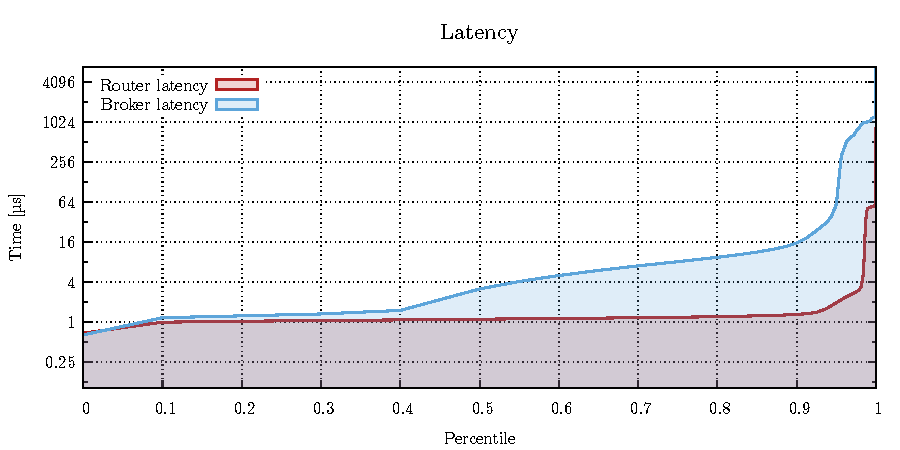
\includegraphics[width=1\linewidth]{obrazky-figures/charts-excel/latency.pdf}
	\caption{Latency chart showing the difference between router and broker latency at 80\,\% of maximum rate. The router's latency is significantly better than latency of Broker.}
	\label{fig:latency}
\end{figure}

Another interesting comparison is between the latency of single instance router and broker. In the Figure~\ref{fig:latency_single} you can see the latency output from the test with the same load of 70\,000 messages per second. Broker can reach this rate with additional queue settings. This configuration improves the distribution of incoming load between multiple queues. That causes that Broker is slightly faster than the router in 40\% cases, but even with that, router is faster in other cases. Router latency has threshold around 60\,$\mu$s, while Broker's has threshold over 1\,000\,$\mu$s. The conclusion is, that router should be much faster than Broker during certain circumstances.

\begin{figure}[h]
	\centering
	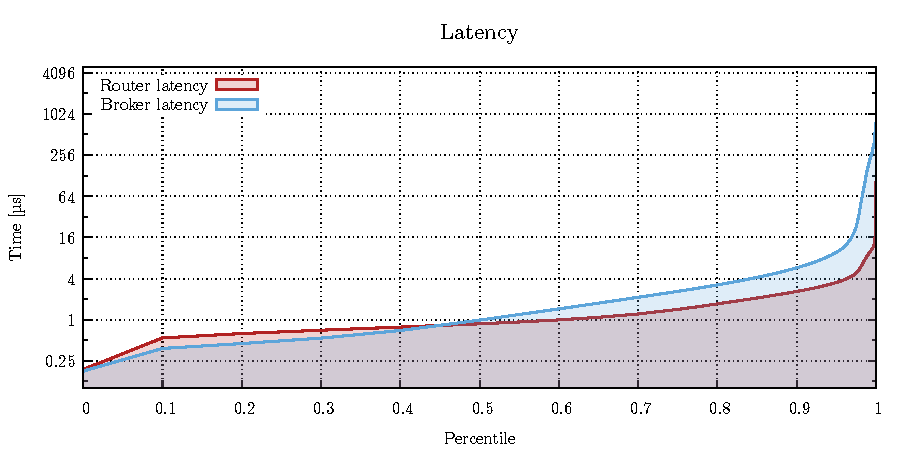
\includegraphics[width=1\linewidth]{obrazky-figures/charts-excel/latency_single.pdf}
	\caption{Router and broker latency comparison during the same load. You can see that router's latency is more stable than latency of Broker.}
	\label{fig:latency_single}
\end{figure}


\section{Behavior Measurements}
\label{Behavior Measurements}

\todo{Tohle popsat az s nejakym dalsim merenim, zatim asi netreba kontrlovat, pouze prevzato z Excelu}

\subsection{Agent Evaluation}
Moreover, I will present some preliminary results with using the agent extension and changing behavior of topology depicted in the Figure \ref{fig:basic_topologies}. In the Figure \ref{fig:agent_throughput} you can see throughput of few simple tests during which middle router is restarted or shut down. The throughput spikes are caused by these events. Since router does not have any queues to store messages, the messages are then discarded and lost. However, the sender does not receive acknowledgment of lost messages so it is not router responsibility. In the Table \ref{tab:agent_simple} you can see the duration of each executed operation and rate of lost messages during the operation (with expected amount of messages being 10\,000\,000). For example during the restart, router was completely shutdown for a second during which no messages arrived. However, after the restart there was some time to balance the load to the previous point. This leads to message lost equals to 2 seconds rate.

% Please add the following required packages to your document preamble:
% \usepackage[table,xcdraw]{xcolor}
% If you use beamer only pass "xcolor=table" option, i.e. \documentclass[xcolor=table]{beamer}
\begin{table}[h]
\centering
\caption{Summarization of lost messages during the connection issues.}
\label{my-label}
\begin{tabular}{|c|r|r|}
\hline
\rowcolor[HTML]{C5E3DF}
Operation     & Duration (seconds) & Message Lost \\ \hline
None          & 0        & None         \\ \hline
Restart       & 1        & 46437        \\ \hline
Shutdown      & 12       & 280572       \\ \hline
Long Shutdown & 89       & 1304451      \\ \hline
\end{tabular}
\label{tab:agent_simple}
\end{table}

The Figure \ref{fig:agent_throughput} also shows, that test case with long shutdown is longer about 10 seconds that other scenarios and the throughput after the shutdown is quite higher. This means that router high throughput to even the messages lost.

\begin{figure}[h]
	\centering
	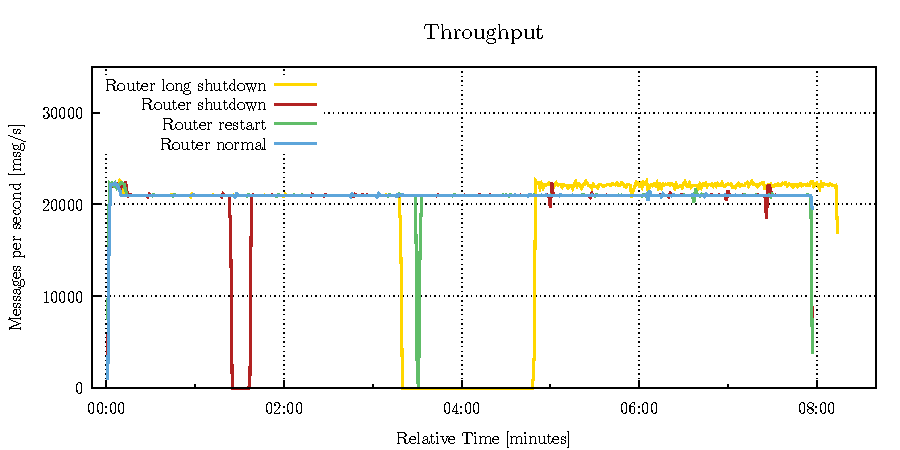
\includegraphics[width=1\linewidth]{obrazky-figures/charts-excel/agent.pdf}
	\caption{Router throughput comparison during the same load after different unexpected events.}
	\label{fig:agent_throughput}
\end{figure}

Latency of test cases cases with the agent function demonstration is depicted in the Figure \ref{fig:agent_latency}. You can see that router is able to even the latency during the restart and short shutdown with test run without any unexpected behavior. On the other hand, long shutdown (red) gets worse latency almost for 50 percentile of messages.

\begin{figure}[h]
	\centering
	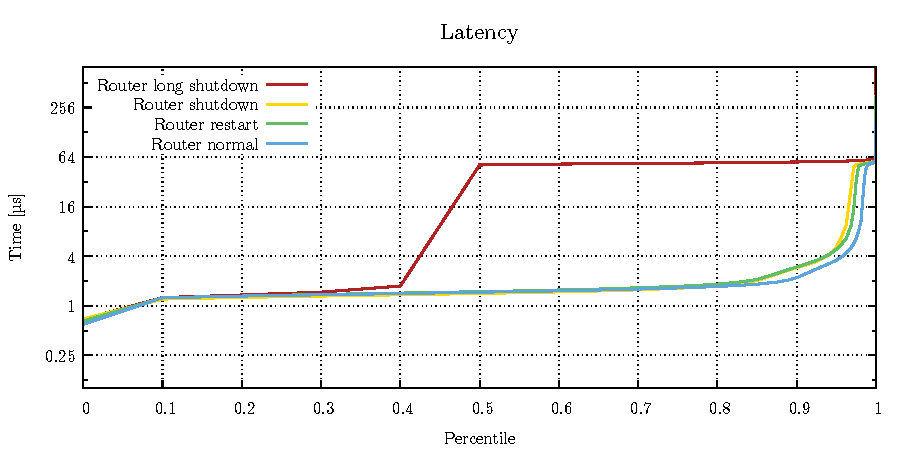
\includegraphics[width=1\linewidth]{obrazky-figures/charts-excel/agent_latency.pdf}
	\caption{Router and broker latency comparison during the same load.}
	\label{fig:agent_latency}
\end{figure}

\section{Performance Testing on Various Generated Topology}

\section{Testing results}
